\documentclass{beamer}
\usepackage{marvosym}
\usepackage{lato}
\usepackage{amsmath, amsfonts, epsfig, xspace}
\usepackage{algorithm,algorithmic}
\usepackage{pstricks,pst-node}
\usepackage{moreverb}
\usepackage[normal,tight,center]{subfigure}


\definecolor{UniBlue}{RGB}{43,61,81}
\definecolor{UniBlueHL}{RGB}{67,98,129}
\definecolor{UniGreen}{RGB}{54,188,123}

\renewcommand*{\familydefault}{fla}
\renewcommand*{\sfdefault}{fla}

\newcommand\bgon{\setbeamertemplate{background}{\parbox[b][17cm]{\paperwidth}{%
\vfill
\includegraphics[height=2.5cm]{logo_alt.pdf}\vfill}}}
\newcommand\bgoff{\setbeamertemplate{background}{}}

\setbeamercolor{title}{fg=white}
\setbeamercolor{frametitle}{fg=UniGreen}
\setbeamercolor{structure}{fg=white}
\setbeamercolor{normal text}{fg=white}
\setbeamercolor{background canvas}{bg=UniBlue}

\begin{document}
\fontseries{l}\selectfont

\title{Migen}
\subtitle{A Python toolbox for building complex digital hardware}
\author{\fontseries{el}\selectfont S\'ebastien Bourdeauducq}
\date{\fontseries{el}\selectfont 2013}

\frame{\titlepage}

\begin{frame}
\begin{centering}

\includegraphics[width=5cm]{migen_logo.png} \\

\includegraphics[width=\textwidth]{migenblock.png}
\end{centering}
\end{frame}

\bgon

\begin{frame}[fragile]
\frametitle{FHDL}
\begin{itemize}
\item Python as a meta-language for HDL
\begin{itemize}
\item Think of a \verb!generate! statement on steroids
\end{itemize}
\item Restricted to locally synchronous circuits (multiple clock domains are supported)
\item Designs are split into:
\begin{itemize}
\item synchronous statements $\Longleftrightarrow$ \verb!always @(posedge clk)! \\
(VHDL: \verb!process(clk) begin if rising_edge(clk) then!)
\item combinatorial statements $\Longleftrightarrow$ \verb!always @(*)! \\
(VHDL: \verb!process(all inputs) begin!)
\end{itemize}
\item Statements expressed using nested Python objects
\begin{itemize}
\item Various syntax tricks to make them look nicer \\
\textit{("internal domain-specific language")}
\end{itemize}
\end{itemize}
\end{frame}

\bgoff
\begin{frame}[fragile]
\frametitle{FHDL crash course}
\begin{itemize}
\item Basic element is \verb!Signal!.
\begin{itemize}
\item Similar to Verilog \verb!wire/reg! and VHDL \verb!signal!.
\end{itemize}
\item Signals can be combined to form expressions.
\begin{itemize}
\item e.g. \verb!(a & b) | c!
\item arithmetic also supported, with user-friendly sign extension rules (\`a la MyHDL)
\end{itemize}
\item Signals have a \verb!eq! method that returns an assignment to that signal.
\begin{itemize}
\item e.g. \verb!x.eq((a & b) | c)!
\end{itemize}
\item User gives an execution trigger (combinatorial or synchronous to some clock) to assignments, and makes them part of a \verb!Module!.
\begin{itemize}
\item Control structures (\verb!If!, \verb!Case!) also supported.
\end{itemize}
\item Modules can be converted for synthesis or simulated.
\end{itemize}
\end{frame}
\bgon

\begin{frame}[fragile]
\frametitle{Conversion for synthesis}
\begin{itemize}
\item FHDL is entirely convertible to synthesizable Verilog
\end{itemize}
\begin{verbatimtab}
>>> from migen.fhdl.std import *
>>> from migen.fhdl import verilog
>>> counter = Signal(16)
>>> o = Signal()
>>> m = Module()
>>> m.comb += o.eq(counter == 0)
>>> m.sync += counter.eq(counter + 1)
>>> print(verilog.convert(m, ios={o}))
\end{verbatimtab}
\end{frame}

\bgoff
\begin{frame}[fragile]
\begin{verbatimtab}
module top(input sys_rst, input sys_clk, output o);

reg [15:0] counter;

assign o = (counter == 1'd0);

always @(posedge sys_clk) begin
        if (sys_rst) begin
                counter <= 1'd0;
        end else begin
                counter <= (counter + 1'd1);
        end
end

endmodule
\end{verbatimtab}
\end{frame}
\bgon

\begin{frame}[fragile]
\frametitle{Name mangling}
\begin{itemize}
\item Problem: how to map the structured Python \verb!Signal! namespace to the flat Verilog namespace?
\item Keep the generated code readable (e.g. for debugging or reading timing reports)
\item Migen uses Python bytecode analysis and introspection to generate (often) meaningful names
\end{itemize}
\end{frame}

\begin{frame}[fragile]
\frametitle{Name mangling in action}
\begin{verbatimtab}
class Foo:
    def __init__(self):
        self.la = [Signal() for x in range(2)]
        self.lb = [Signal() for x in range(3)]
a = [Foo() for x in range(3)]
\end{verbatimtab}

$\rightarrow$ foo0\_la0, foo0\_la1, foo0\_lb0, foo0\_lb1, foo1\_la0, ...,
  foo1\_lb0, ..., foo2\_lb2
\end{frame}

\begin{frame}
\centering 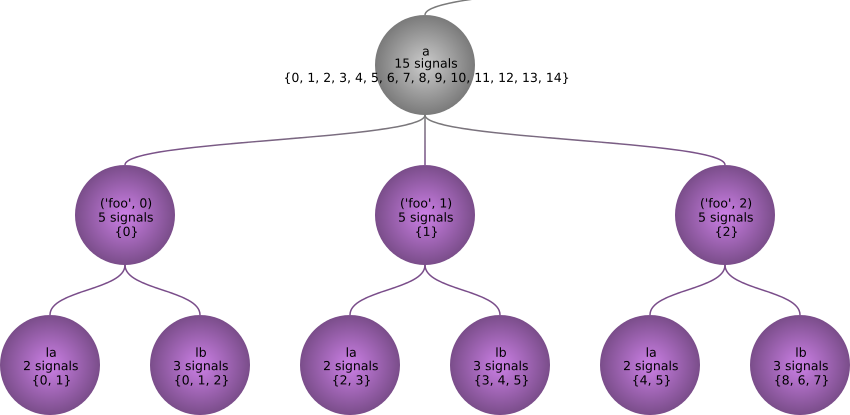
\includegraphics[width=\textwidth]{name_mangling.png}
\end{frame}

\begin{frame}[fragile]
\frametitle{Simulation}
\begin{itemize}
\item Modules can have a Python functions to execute at each clock cycle during simulations.
\item Simulator provide read and write methods that manipulate FHDL \verb!Signal! objects.
\item Python libraries useful for DSP testbenches: scipy, matplotlib
\item Python makes it easy to run multiple simulations with different parameters (including changes of IO timings)
\item Writing self-checking testbenches is straightforward: reproduciblity, reusability
\end{itemize}
\end{frame}

\bgoff
\begin{frame}[fragile]
\frametitle{Simulation}
\begin{itemize}
\item Powerful Python features, e.g. generators:
\end{itemize}
\begin{verbatimtab}
def my_generator():
        for x in range(10):
                t = TWrite(x, 2*x)
                yield t
                print("Latency: " + str(t.latency))
                for delay in range(prng.randrange(0, 3)):
                        yield None # inactivity
master1 = wishbone.Initiator(my_generator())
master2 = lasmibus.Initiator(my_generator(), port)
\end{verbatimtab}
\end{frame}

\begin{frame}[fragile]
\frametitle{Pytholite}
\begin{itemize}
\item Some of those generators are even synthesizable :)
\item Output: FSM + datapath
\item Lot of room for improvement (mapping, scheduling, recognized subset)
\item One application today: high-speed control of the analog RF chain of a radar
\end{itemize}
\begin{verbatimtab}
def generator():
        for i in range(10):
                yield TWrite(i, 0)
bus_if = wishbone.Interface()
pl = make_pytholite(generator,
        buses={"def": bus_if})
... verilog.convert(pl) ...
\end{verbatimtab}
\end{frame}
\bgon

\begin{frame}[fragile]
\frametitle{Bus support}
\begin{itemize}
\item Wishbone\footnote{http://www.opencores.org}
\item SRAM-like CSR
\item DFI \footnote{http://www.ddr-phy.org}
\item LASMI
\end{itemize}
\centering 
\includegraphics[height=1cm]{opencores.png} 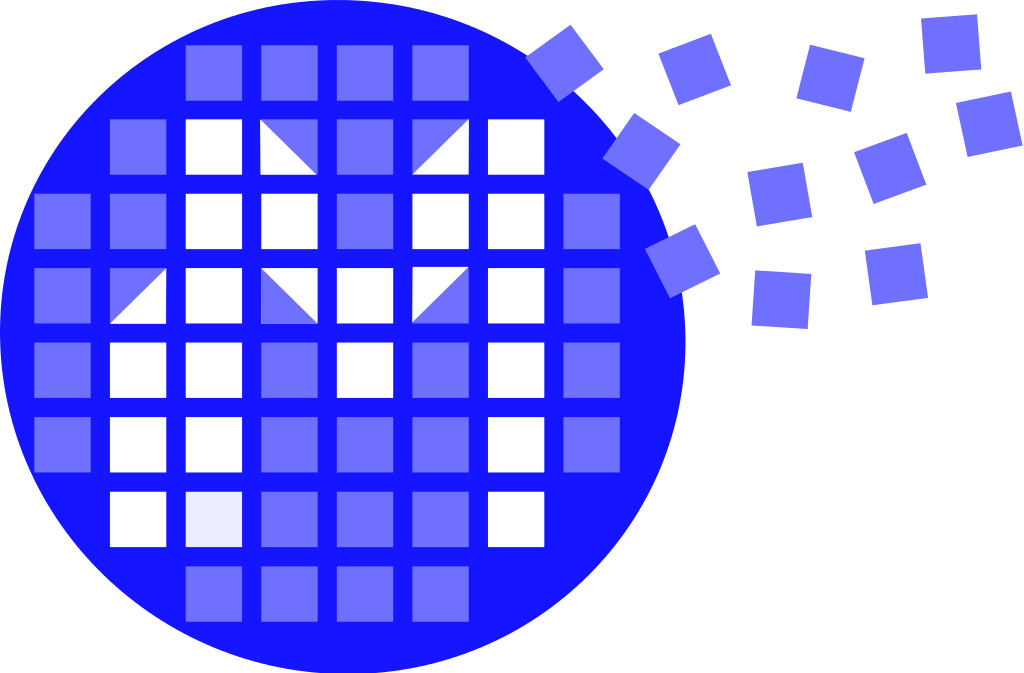
\includegraphics[height=1cm]{milkymist.png} 
\includegraphics[height=1cm]{dfi.png}
\begin{verbatimtab}
wishbonecon0 = wishbone.InterconnectShared(
        [cpu0.ibus, cpu0.dbus],
        [(lambda a: a[26:29] == 0, norflash0.bus),
         (lambda a: a[26:29] == 1, sram0.bus),
         (lambda a: a[26:29] == 3, minimac0.membus),
         (lambda a: a[27:29] == 2, wishbone2lasmi0.wb),
         (lambda a: a[27:29] == 3, wishbone2csr0.wb)])
\end{verbatimtab}
\end{frame}

\begin{frame}[fragile]
\frametitle{CSR banks}
Migen user:
\begin{verbatimtab}
self.baudrate = CSRStorage(16)
... If(counter == 0,
  counter.eq(self.baudrate.storage))
...
\end{verbatimtab}
Migen generates address decoder and register logic. \\
Rhino-gateware does BORPH interfacing. \\
$\rightarrow$ Software user:
\begin{verbatimtab}
/proc/[pid]/hw/ioreg/baudrate
\end{verbatimtab}
\end{frame}

\begin{frame}
\frametitle{LASMI}
LASMI (Lightweight Advanced System Memory Infrastructure) key ideas
\begin{itemize}
\item Speed is beautiful: optimize for performance
\item Operate several FSMs (\textit{bank machines}) concurrently to manage each bank
\item Crossbar interconnect between masters and bank machines
\item Pipelining: new requests can be issued without waiting for data. Peak IO bandwidth (minus refresh) is attainable.
\item In a frequency-ratio system, issue multiple DRAM commands from different bank FSMs in a single cycle
\end{itemize}
\end{frame}

\begin{frame}
\frametitle{LASMIcon (MiSoC)}
Memory controller operates several \textit{bank machines} in parallel
\begin{itemize}
\item Each bank machine uses the page mode algorithm
\item Tracks open row, detects page hits
\item Ensures per-bank timing specifications are met (tRP, tRCD, tWR)
\item Generates DRAM-level requests (PRECHARGE, ACTIVATE, READ, WRITE)
\end{itemize}
\end{frame}

\bgoff
\begin{frame}
\frametitle{LASMIcon (MiSoC)}
\textit{Command steering} stage picks final requests
\begin{itemize}
\item In a frequency-ratio system, may issue multiple commands from several bank machines in a single cycle
\begin{itemize}
\item PHY uses SERDES to handle I/O
\item FPGAs are horribly and painfully SLOW, so we need such tricks even for DDR333 (2002!!!)
\end{itemize}
\item Groups writes and reads to reduce turnaround times (reordering)
\begin{itemize}
\item commands stay executed in-order for each bank machine: no reorder buffer needed on the master side
\end{itemize}
\item Ensures no read-to-write conflict occurs on the shared bidirectional data bus
\item Ensures write-to-read (tWTR) specification is met
\end{itemize}
\end{frame}
\bgon

\begin{frame}
\frametitle{LASMIcon (MiSoC)}
\begin{itemize}
\item Supports SDR, DDR, LPDDR, DDR2 and DDR3
\item Hardware tested:
\begin{itemize}
\item Mixxeo digital video mixer (Spartan-6, DDR, 10Gbps)
\item Experiment control board from Paul-Drude-Institut Berlin (Spartan-6, DDR2, 4Gbps)
\item FPGA development boards: KC705 (Kintex-7, DDR3), LX9 Microboard (Spartan-6, LPDDR), Altera DE0Nano (Cyclone, SDR), ...
\end{itemize}
\end{itemize}
\end{frame}

\begin{frame}
\frametitle{Dataflow programming}
\begin{itemize}
\item Representation of algorithms as a graph (network) of functional units
\item Similar to Simulink or LabVIEW
\item Parallelizable and relatively intuitive
\item Migen provides infrastructure for actors (functional units) written in FHDL
\item Migen provides an actor library for DMA (Wishbone and LASMI), simulation, etc.
\end{itemize}
\end{frame}

\bgoff

\begin{frame}
\frametitle{DF example: Fourier transform}
\begin{centering}
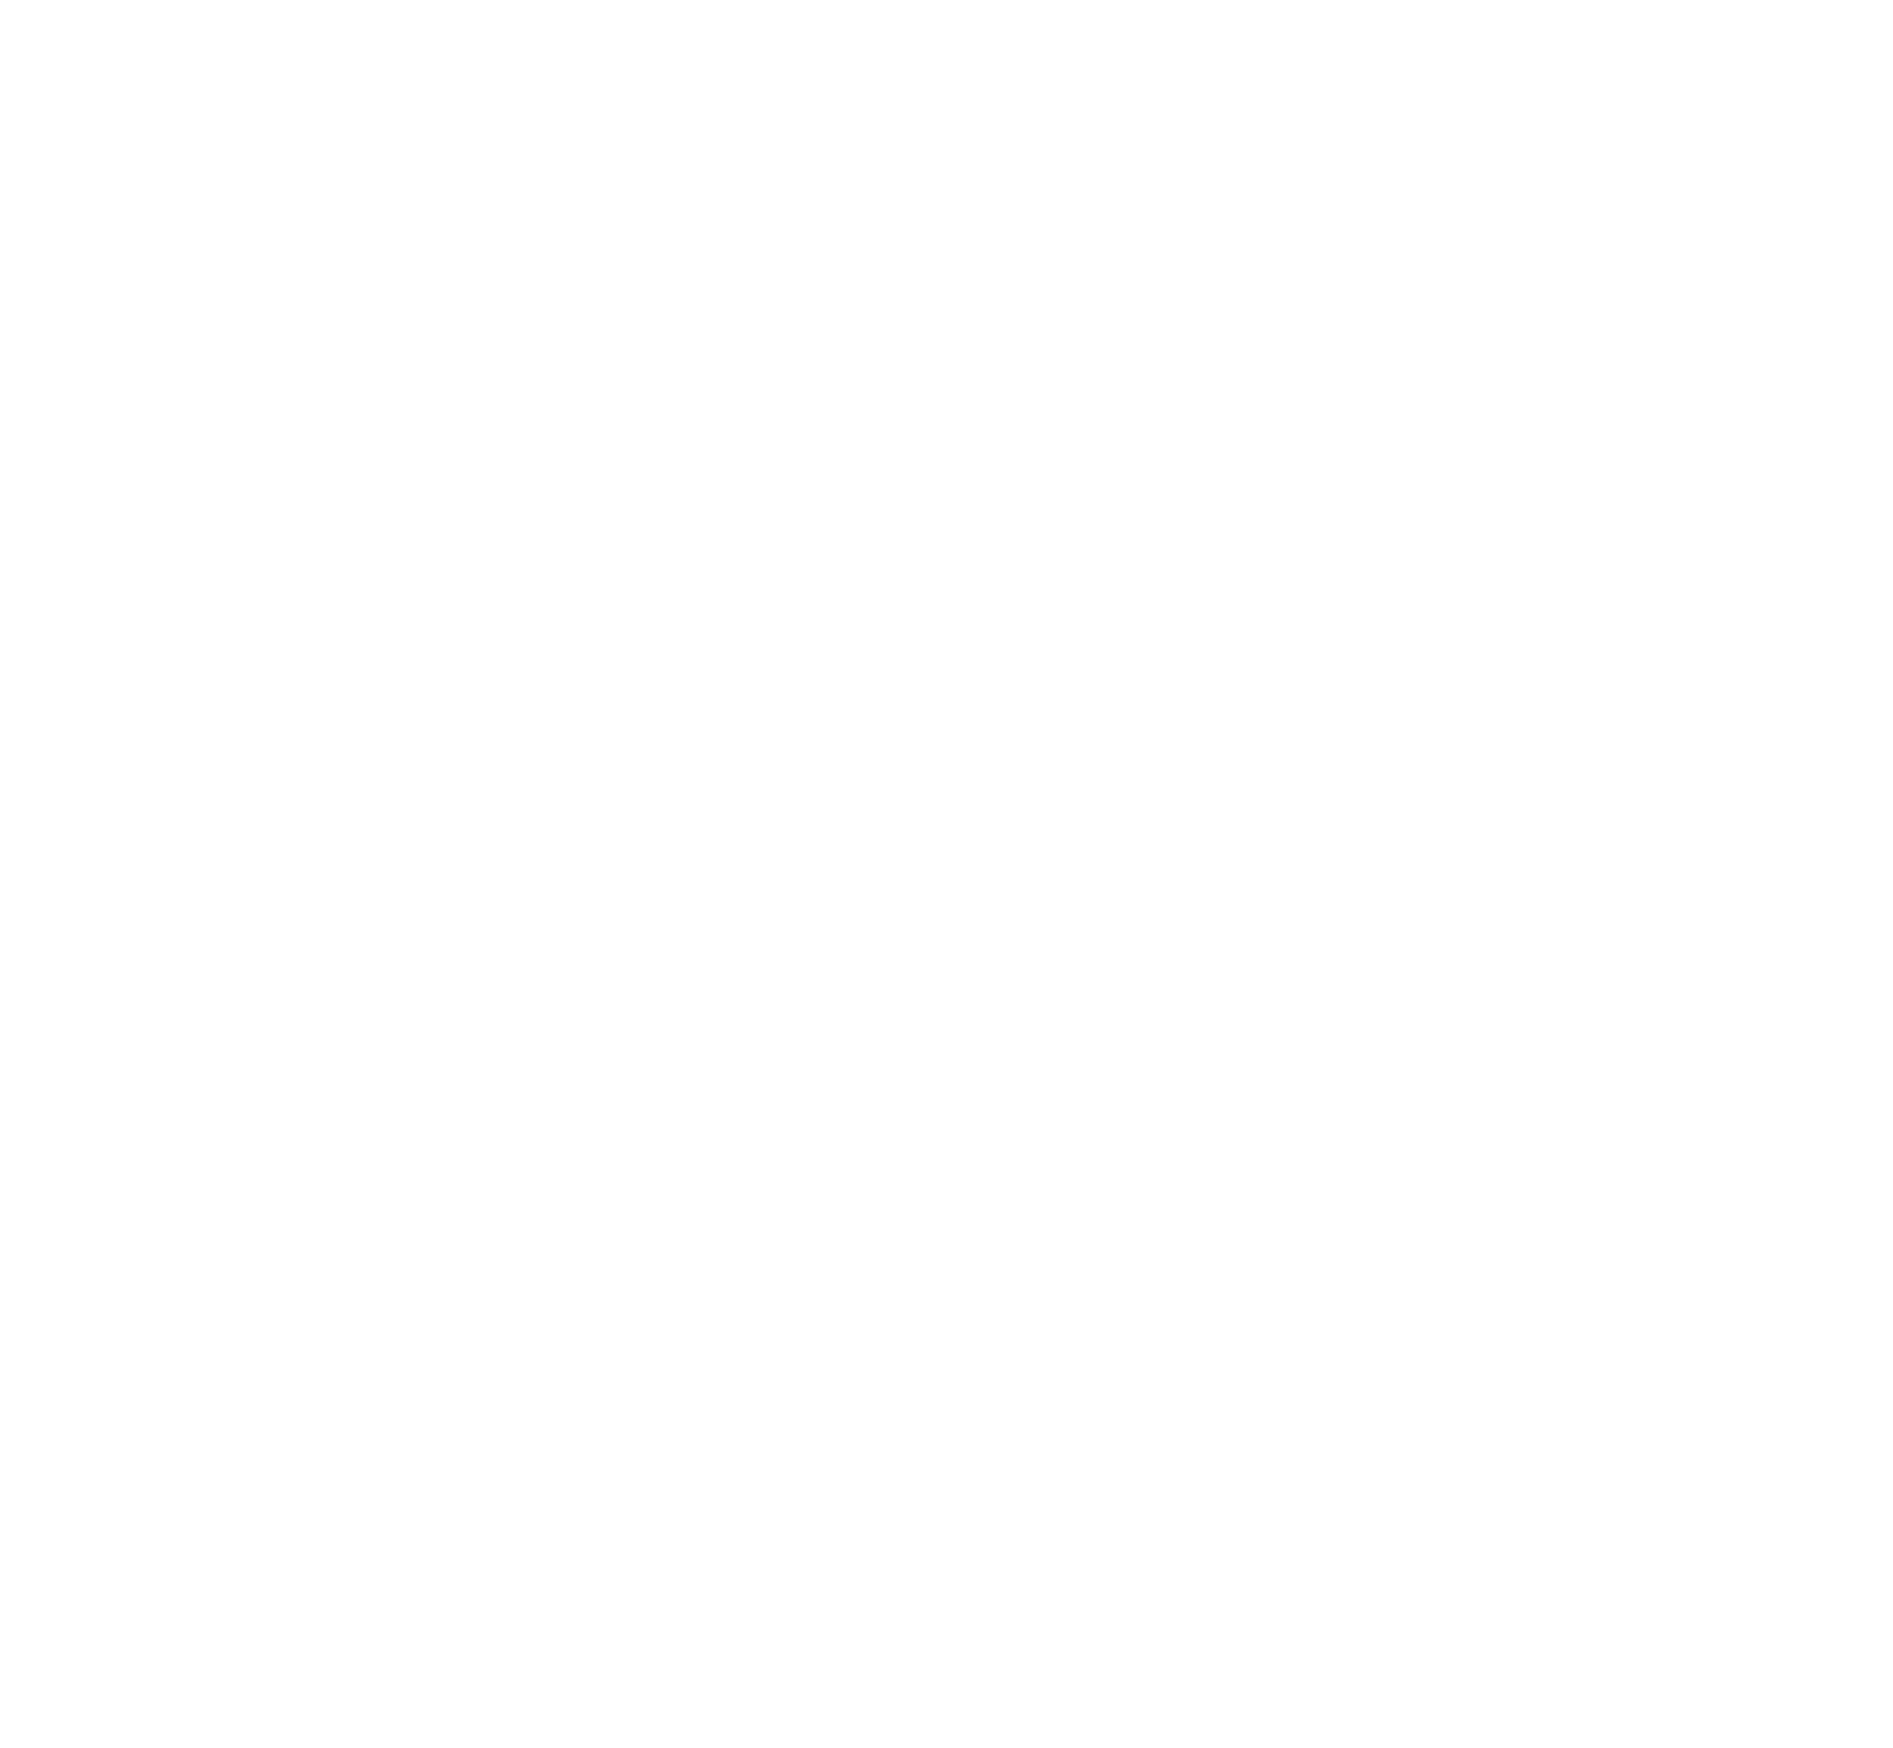
\includegraphics[width=8cm]{fft.png}
\end{centering}

\small Graph by C. Burrus ``FFT Flowgraphs'' \url{http://cnx.org/content/m16352/latest/}
\end{frame}

\bgon
\begin{frame}[fragile]
\frametitle{Mibuild}
Interface between Migen and your FPGA board
\begin{verbatimtab}
from mibuild.platforms import roach
plat = roach.Platform()
m = YourModule(plat.request("clocks"),
  plat.request("adc"), plat.request("dac"))
plat.build_cmdline(m)
\end{verbatimtab}
\begin{itemize}
\item Supports Xilinx: ISE and Vivado (including 7 series)
\item Supports Altera: Quartus
\item Runs on Linux and Windows
\end{itemize}
\end{frame}

\begin{frame}
\frametitle{Current Migen users}
\begin{itemize}
\item Mixxeo digital video mixer
\item RHINO --- software-defined radio
\item Vermeer --- radar
\item NIST --- trapped ion quantum computers
\item Paul-Drude-Institut Berlin --- experiment control
\item A few semiconductor companies --- ??? (fixing bugs)
\item OpenVizsla Open Hardware FPGA-based USB analyzer
\item Miscope -- Small logic analyzer embedded in the FPGA
\item PCIe Software Defined Radio board with Artix 7
\item SATA controller for Xilinx 7-series FPGAs
\end{itemize}
\end{frame}

\begin{frame}
\frametitle{Current and future works}
\begin{itemize}
\item Dataflow system overhaul
\begin{itemize}
\item Static scheduling when possible
\item Actor sharing
\item Better graph language
\item Unify with Pytholite?
\end{itemize}
\item GUI
\begin{itemize}
\item Build simple DF graphs more easily
\item For complex designs, Python programming is great
\end{itemize}
\item Direct synthesis (Mist): Migen FHDL to EDIF netlist
\begin{itemize}
\item Get rid of the Xst proprietary bloatware
\item Later: get rid of the P\&R + Bitgen proprietary bloatware
\end{itemize}
\end{itemize}
\end{frame}

\begin{frame}
\frametitle{Direct synthesis (Mist)}
\begin{itemize}
\item Right now
\begin{itemize}
\item basic logic operations
\item registers
\item IO
\item instantiation of pre-existing IP
\end{itemize}
\item Working on
\begin{itemize}
\item Arithmetic operations
\item BRAM
\end{itemize}
\item To Do
\begin{itemize}
\item Optimization
\end{itemize}
\end{itemize}
\end{frame}

\bgoff

\begin{frame}
Migen is open source!
\begin{itemize}
\item BSD license
\begin{itemize}
\item Compatible with proprietary designs.
\item Contributing what you can is \textit{encouraged}.
\end{itemize}
\item http://m-labs.hk/gateware.html
\item http://github.com/m-labs/migen
\item Mailing lists: http://lists.m-labs.hk $=>$ Devel
\item IRC: Freenode \#m-labs (formerly known as \#milkymist)
\item Commercial support available
\end{itemize}

\centering 
\includegraphics[width=5cm]{migen_logo.png}

\end{frame}

\end{document}
